\section{Dataset}
Il dataset \cite{ni2019justifying} utilizzato in questo lavoro contiene i prodotti e le recensioni di Amazon dal 1999 fino al 2018 raggruppate
in macro-categorie.
Per esigenze computazionali il dataset è stato ridotto selezionando casualmente 30,000 recensioni dalla sotto-categoria \textit{Internal Components}.

Nelle tabelle \ref{tab:attr-products} e \ref{tab:attr-reviews} vengono rispettivamente descritti tutti gli attributi dei prodotti e delle recensioni forniti. In questo lavoro sono stati analizzati e utilizzati solo i seguenti attributi: \textit{asin}, \textit{title}, \textit{description}, \textit{brand}, \textit{price}, \textit{categories}, \textit{imageURLHighRes}, \textit{reviewText}, \textit{vote}, \textit{overall}, \textit{summary} e \textit{unixReviewTime}.

Per semplicità gli attributi \textit{reviewText}, \textit{unixReviewTime} sono stati rinominati rispettivamente in \textit{text}, \textit{timestamp}.

\begin{table}[ht]
\centering
\begin{tabular}{|p{3.5cm}|p{7.5cm}|}
\hline
\textbf{asin}             & ID del prodotto                                                    \\ \hline
\textbf{title}            & nome del prodotto                                                  \\ \hline
\textbf{description}      & descrizione del prodotto                                           \\ \hline
\textbf{brand}            & marchio                                                            \\ \hline
\textbf{date}             & data di disponibilità                                              \\ \hline
\textbf{price}            & prezzo in dollari (al tempo di crawl)                              \\ \hline
\textbf{main{\_}cat}      & categoria principale del prodotto                                  \\ \hline
\textbf{categories}       & lista delle categorie a cui appartiene                             \\ \hline
\textbf{imageURL}         & URL delle immagini                                                 \\ \hline
\textbf{imageURLHighRes}  & URL delle immagini ad alta risoluzione                             \\ \hline
\textbf{rank}             & informazioni sul ranking di vendita                                \\ \hline
\textbf{feature}          & lista di caratteristiche del prodotto                              \\ \hline
\textbf{details}          & dettagli del prodotto                                              \\ \hline
\textbf{tech1}            & prima tabella dei dettagli tecnici del prodotto                    \\ \hline
\textbf{tech2}            & seconda tabella dei dettagli tecnici del prodotto                  \\ \hline
\textbf{also{\_}view}     & prodotti anche visti                                               \\ \hline
\textbf{also{\_}buy}      & prodotti anche acquistati                                          \\ \hline
\textbf{similar{\_}item}  & prodotti simili                                                    \\ \hline
\end{tabular}
\caption{Attributi dei prodotti}
\label{tab:attr-products}
\end{table}

\begin{table}[ht]
\centering
\begin{tabular}{|p{3.5cm}|p{7.5cm}|}
\hline
\textbf{reviewerID}     & ID del recensore                                    \\ \hline
\textbf{asin}           & ID del prodotto                                     \\ \hline
\textbf{reviewerName}   & nome del recensore                                  \\ \hline
\textbf{verified}       & recensione con acquisto verificato                  \\ \hline
\textbf{vote}           & \#utenti che hanno trovato utile la recensione      \\ \hline
\textbf{style}          & metadati del prodotto                               \\ \hline
\textbf{reviewText}     & testo della recensione                              \\ \hline
\textbf{overall}        & valutazione del prodotto (da 1 a 5)                 \\ \hline
\textbf{summary}        & breve descrizione della recensione                  \\ \hline
\textbf{unixReviewTime} & tempo della recensione (unix)                       \\ \hline
\textbf{reviewTime}     & tempo della recensione (raw)                        \\ \hline
\textbf{image}          & immagini del prodotto postate dall'utente           \\ \hline
\end{tabular}
\caption{Attributi delle recensioni}
\label{tab:attr-reviews}
\end{table}

Per prima cosa è stata effettuata una pulizia dei dati per alcuni attributi rimuovendo eventuali parti di codice HTML/CSS.

Per l'attributo \textit{price} sono stati rimossi il simbolo \$ e le virgole che separano le migliaia. I valori con lunghezza uguale a 0 o superiore a 8 sono stati considerati non validi.

Dall'attributo \textit{categories} sono state estratte le sotto-categorie di \textit{Internal Components} e sono state rinominate rimuovendo la parola \textit{Internal} che è già implicita nella sotto-categoria scelta in questo lavoro.

Per l'attributo \textit{brand} inoltre è stata effettuata una normalizzazione tramite le seguenti operazioni, riducendo il numero di \textit{brand} unici da 2842 a 828:
\begin{enumerate}
  \item minuscolo
  \item rimozione dei seguenti caratteri: ``.'', ``,'', ``\{'', ``\}''
  \item rimozione spazi in eccesso
  \item rimozione delle seguenti parole: ``by'', ``limited'', ``llc'', ``ltd'', ``inc'', ``co'', ``corp'', ``corporated'', ``corporation''
  \item rinominazione dei brand composti da 1 solo carattere o da più di 7 parole in ``unknown''
\end{enumerate}

Successivamente sono stati identificati i valori mancanti e duplicati.
%
Nella figura \ref{fig:missing_values} sono state riportate le percentuali dei valori mancanti per ogni attributo.
Gli unici attributi con valori mancanti sono \textit{description}, \textit{imageURLHighRes} e \textit{price}. Questi attributi
prima della pulizia presentavano parti di codice HTML/CSS in alcune recensioni, quindi si presume che molti di questi valori non siano
stati estratti correttamente dal \textit{crawler} e sono stati ignorati nel resto dell'analisi.
%
Per quanto riguarda i duplicati sono state trovate e rimosse 67 recensioni con gli attributi \textit{asin}, \textit{summary}, \textit{text} e \textit{overall} uguali.

\begin{figure}[ht]
  \centering
  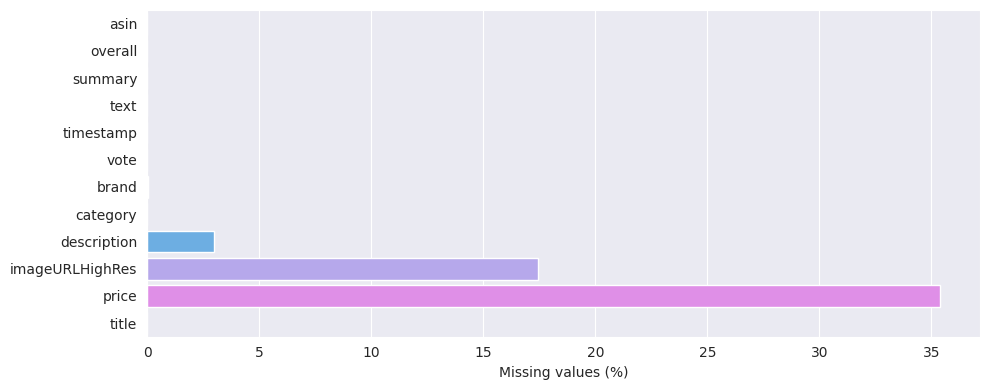
\includegraphics[width=0.95\textwidth]{images/dataset/missing_values.png}
  \caption{Percentuale dei valori mancanti per ogni attributo.}
  \label{fig:missing_values}
\end{figure}

Tramite il modello FastText \cite{joulin2016bag} sono state identificate e mantenute solo le recensioni in lingua inglese considerando l'attributo \textit{text}, in cui sono stati rimossi gli URL e i tag HTML e infine è stato trasformato in minuscolo.
%
Il numero di recensioni rimanenti è 28,983 che corrisponde al 96\% del dataset.

\subsection{Exploratory Data Analysis}
Successivamente sono state effettuate diverse analisi esplorative del dataset pulito.
Inizialmente sono state effettuate delle verifiche per controllare che non fossero presenti casi anomali, ad esempio verificare se un utente avesse fatto tutte le recensioni relative ad un prodotto.

Il dataset presenta un numero di 4,803 prodotti, e 25,374 recensori unici. Il numero medio di recensioni per prodotto è di 6, mentre il numero di recensioni medio per recensore è di 1.

Nella figura \ref{fig:eda_nreviews} viene mostrato il quantitativo di prodotti che possiedono un determinato numero di recensioni. Come si può notare la maggior parte dei prodotti ha al più 5 recensioni.

\begin{figure}[ht]
    \centering
    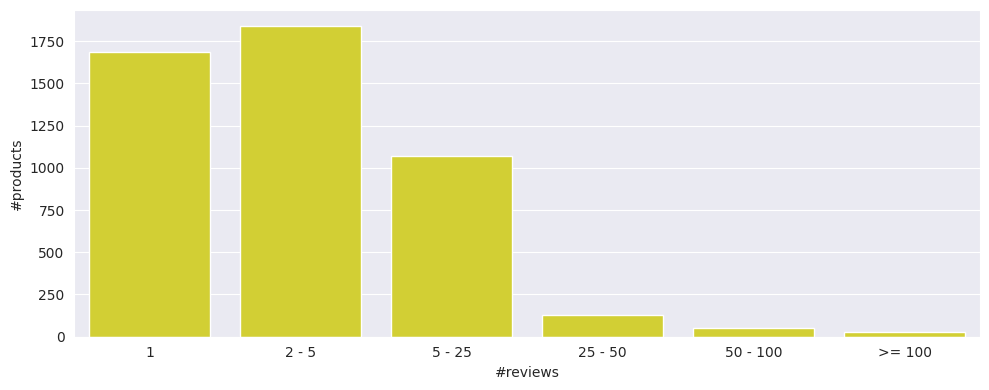
\includegraphics[width=0.9\textwidth]{images/eda/eda_reviews_product_number.png}
    \caption{Numero di prodotti in base alla quantità di recensioni associate.}
    \label{fig:eda_nreviews}
\end{figure}

Successivamente è stato analizzato l'andamento delle recensioni nel tempo (figura \ref{fig:eda_reviews_distribution}), dove si può vedere un aumento considerevole negli ultimi anni probabilmente dovuto alla diffusione dell'utilizzo di Amazon; si trova conferma di questo anche nella figura \ref{fig:eda_number_products} dove viene mostrato il numero di prodotti disponibili nel tempo.

\begin{figure}[ht]
    \centering
    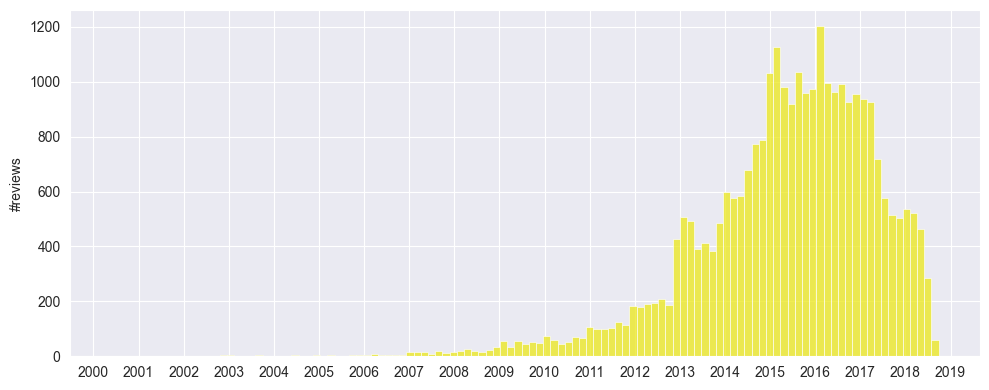
\includegraphics[width=0.95\textwidth]{images/eda/eda_distribuiont_reviews.png}
    \caption{Numero di recensioni nel tempo.}
    \label{fig:eda_reviews_distribution}
\end{figure}

\begin{figure}[p]
    \centering
    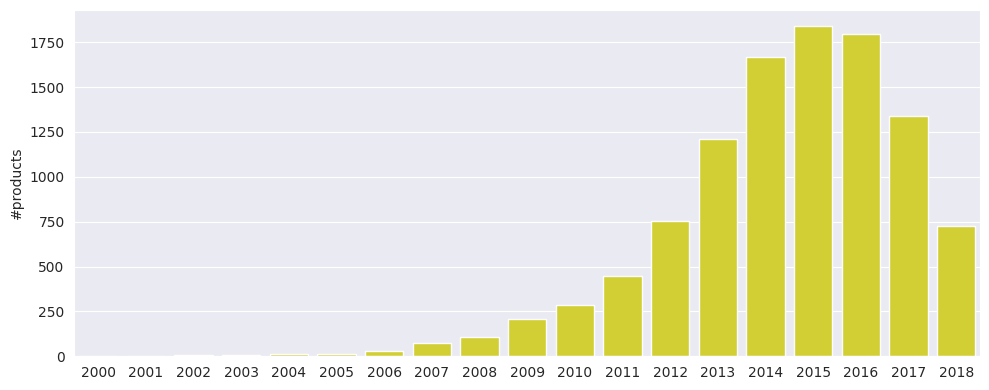
\includegraphics[width=0.8\textwidth]{images/eda/eda_number_products.png}
    \caption{Numero di prodotti per anno.}
    \label{fig:eda_number_products}
\end{figure}


Nelle figura \ref{fig:eda_brand_reviews} viene mostrato il numero di recensioni
per i top-20 brand, mentre nella figura \ref{fig:eda_category_reviews} viene mostrato
il numero di recensioni per categoria del prodotto.

\begin{figure}[p]
    \centering
    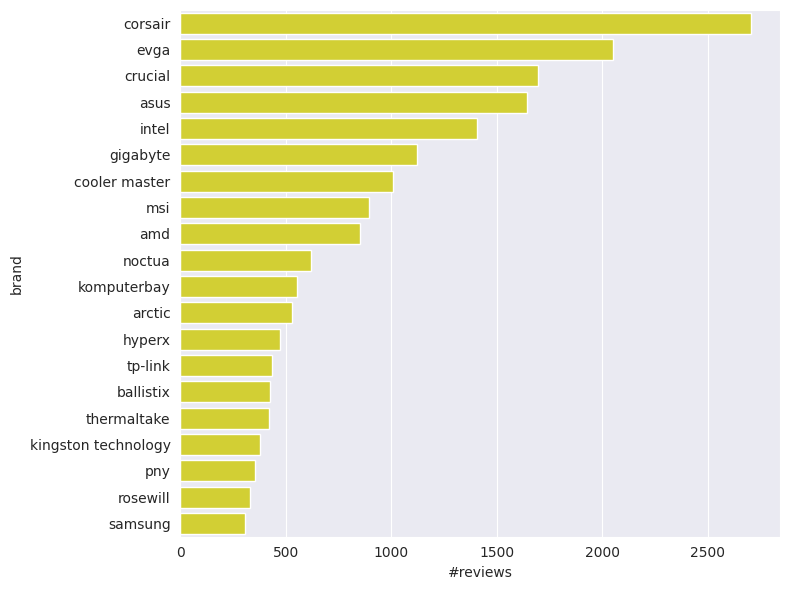
\includegraphics[width=0.65\textwidth]{images/eda/eda_reviews_brand.png}
    \caption{Distribuzione delle recensioni per brand.}
    \label{fig:eda_brand_reviews}
\end{figure}

\begin{figure}[p]
    \centering
    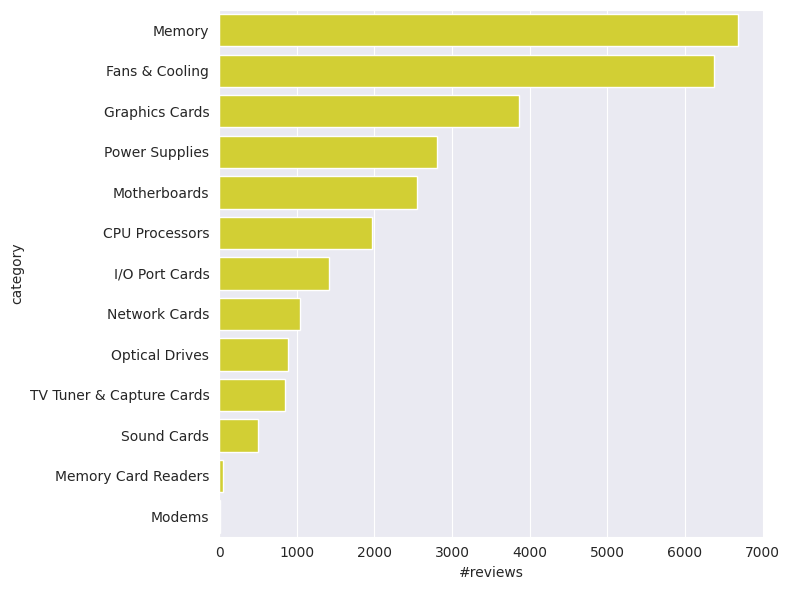
\includegraphics[width=0.7\textwidth]{images/eda/eda_reviews_category.png}
    \caption{Distribuzione delle recensioni per categoria.}
    \label{fig:eda_category_reviews}
\end{figure}

\newpage

Una caratteristica importante da analizzare è il numero di stelle, che fornisce una prima e immediata valutazione del prodotto da parte dell'utente. Nella figura \ref{fig:eda_overall} viene mostrata la loro distribuzione in percentuale. Le recensioni presentano un numero di stelle prevalentemente positivo, infatti più dell'80\% hanno una valutazione tra 4 e 5 stelle.

\begin{figure}[ht]
    \centering
    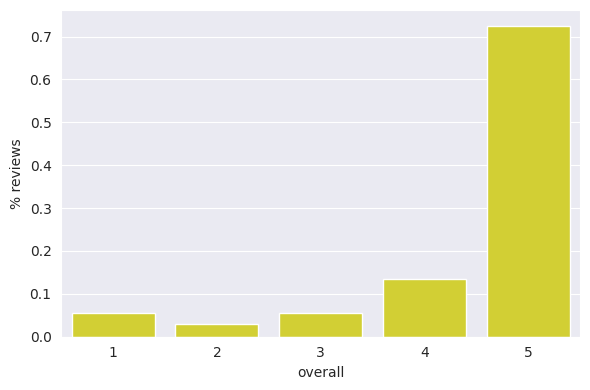
\includegraphics[width=0.7\textwidth]{images/eda/eda_overall.png}
    \caption{Distribuzione delle recensioni per numero di stelle.}
    \label{fig:eda_overall}
\end{figure}

Inoltre è possibile considerare il numero di voti assegnato a una recensione che indica, secondo gli utenti, quanto sia utile. Questo attributo può essere utilizzato per dare un peso alle recensioni, ma osservando la figura \ref{fig:eda_vote} si nota come gli utenti tendano a non votare le recensioni.

\begin{figure}[ht]
    \centering
    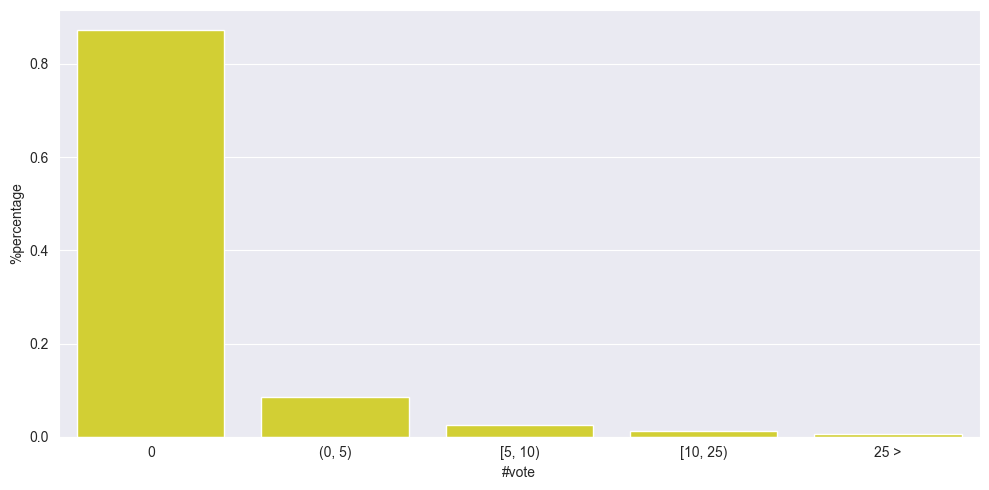
\includegraphics[width=0.8\textwidth]{images/eda/eda_vote.png}
    \caption{Percentuale di recensioni per numero di voti.}
    \label{fig:eda_vote}
\end{figure}

Infine è stata analizzata la parte testuale delle recensioni ovvero titolo e testo. Nelle figure \ref{fig:eda_summary} e \ref{fig:eda_text} viene mostrata la percentuale delle recensioni in base alla lunghezza del titolo e del testo. Per quanto riguarda il titolo
si può notare che più della metà delle recensioni hanno una lunghezza di 10-25 caratteri.

\begin{figure}[ht]
    \centering
    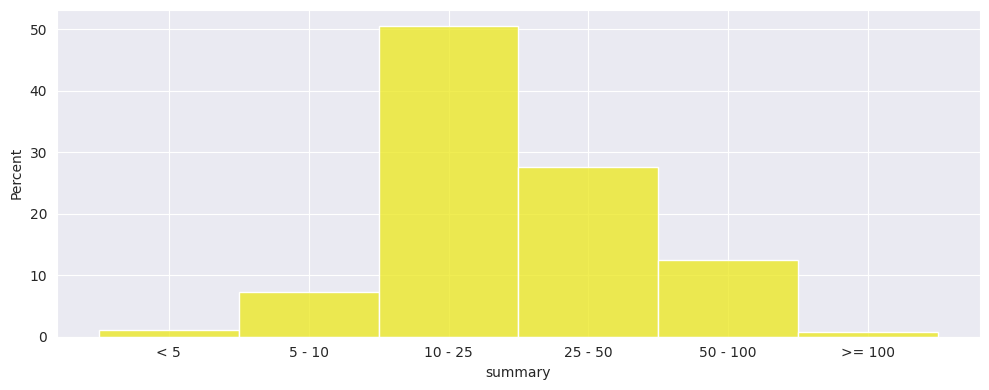
\includegraphics[width=0.95\textwidth]{images/eda/eda_summary.png}
    \caption{Percentuale di recensioni in base alla lunghezza del titolo.}
    \label{fig:eda_summary}
\end{figure}

\begin{figure}[ht]
    \centering
    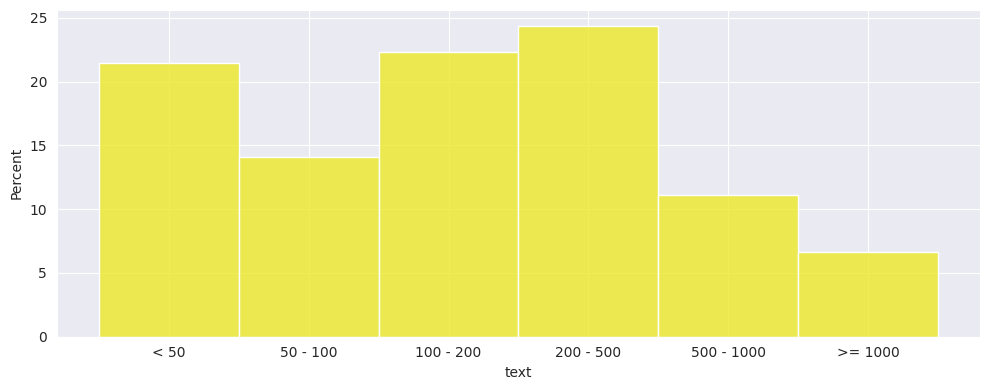
\includegraphics[width=0.95\textwidth]{images/eda/eda_text.png}
    \caption{Percentuale di recensioni in base alla lunghezza del testo.}
    \label{fig:eda_text}
\end{figure}